\documentclass[exercice]{thedocument}%
\usepackage{texmaths-tikz}%
\startdatakeys
\source{}
\cycle{}
\competencesDuSocle{}
\connaissancesRequises{}
\competencesTravaillees{}
\enddatakeys
\begin{document}%
En utilisant les informations données et le codage, calculer le périmètre
de la figure.\par\smallskip\noindent
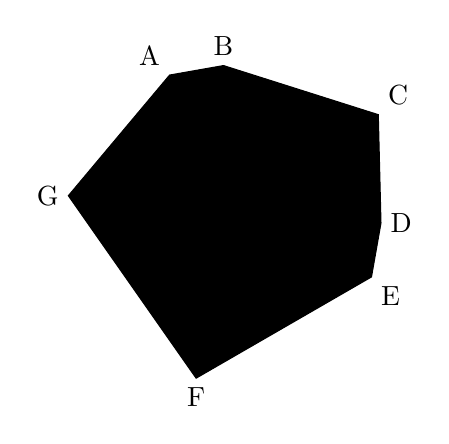
\begin{tikzpicture}[scale=2, baseline=(current bounding box.center)]
    \coordinate[label=right:D](D)at(0:1);
    \coordinate[label=above right:C](C)at(35:1.2);
    \coordinate[label=B](B)at(90:1);
    \coordinate[label=above left:A](A)at(110:1);
    \coordinate[label=left:G](G)at(170:1);
    \coordinate[label=below right:E](E)at(-20:1);
    \coordinate[label=below:F](F)at(-100:1);
    \draw[fill=\currentcolor](G)--(F)--(E)--(D)--(C)--(B)--(A)--cycle;
    \tkzMarkSegments[\maincodagecolor, mark=|](G,F F,E B,C)
    \tkzMarkSegments[\maincodagecolor, mark=||](A,B E,D)
    \tkzMarkSegments[\maincodagecolor, mark=x](C,D G,A)
\end{tikzpicture}\hskip20pt
\begin{minipage}[c]{.3\linewidth}
    \noindent$\text{AB}=0,025\text{ m}$\par
    \noindent$\text{BC}=4,2\text{ cm}$\par
    \noindent$\text{CD}=32,5\text{ dm}$\par
\end{minipage}
\end{document}
